\section{P4D-Bench: Evaluating Navigation in Evolving Worlds}
\label{sec:benchmark}

\pfdbench{} couples longitudinal hidden state changes with executable embodied
episodes across \textbf{54 scenes} and \textbf{803.68k task instances}.
Unlike fixed-scene evaluation, it tests whether an agent can infer the present
from a causal history after an observation gap. Four design constraints preserve
temporal continuity, causal observability, physical executability, and controlled
dynamics: histories persist across queries, public evidence precedes the query,
placements have reachable inspection viewpoints, and paired worlds isolate the
hidden transition mechanism.

\begin{figure}[!htbp]
    \centering
    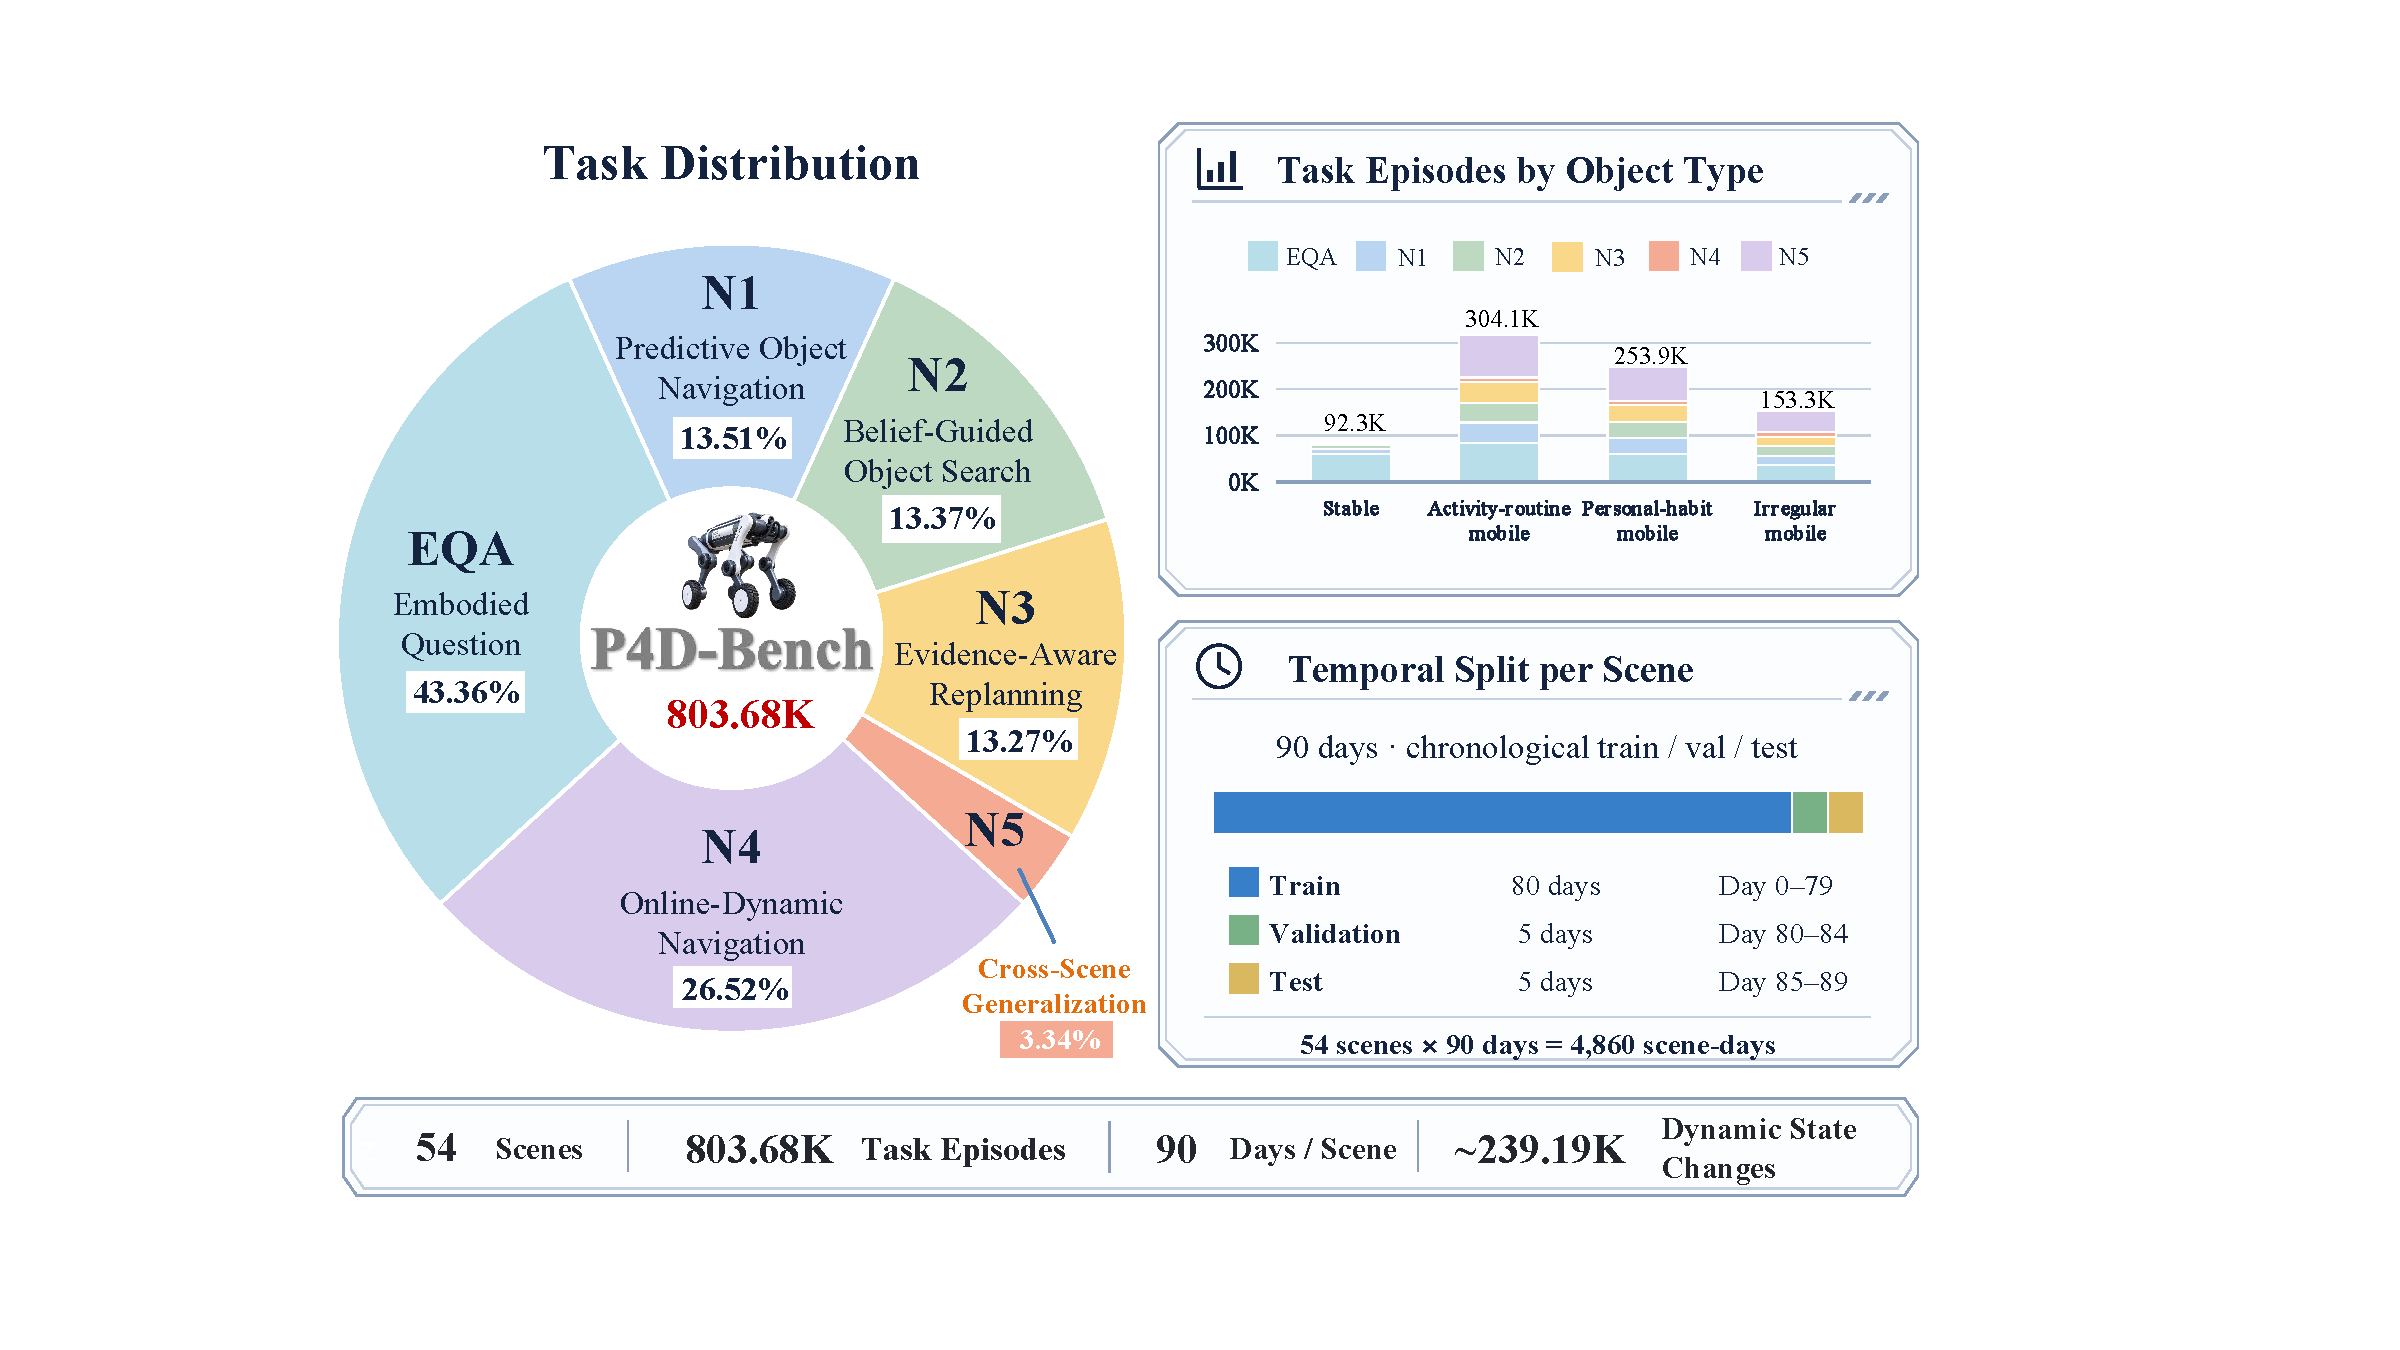
\includegraphics[width=0.80\linewidth]{figures/P4D_Benchmark.pdf}
    \caption{Overview of \pfdbench{} evaluation protocols.}
    \label{fig:p4dbench}
\end{figure}

\paragraph{Task coverage.}
The pool contains current-state prediction (16\%), object navigation (27\%),
vision-and-language navigation (29\%), and embodied question answering (28\%)
\citep{majumdar2024openeqa,sakamoto2024map}.
The experiments emphasize prediction and navigation; EQA diagnoses memory,
while the remaining annotations support broader study.
All tracks share evolving scene histories and causal evidence
(\cref{fig:p4dbench}).

\paragraph{Human-trace-grounded construction.}
We align longitudinal smart-home records from CASAS \citep{cook2013casas} and
ARAS, multi-week activity and object-location sequences from HOMER+
\citep{patel2023routine}, and action--object and placement evidence from HD-EPIC
and ParaHome \citep{perrett2025hdepic,kim2025parahome}, supplemented by
OPPORTUNITY. A common event schema links time, activity, actor context, object,
source and destination states, and provenance. These sources constrain schedules,
activity--object associations, transition timing, and placement tendencies;
trajectories are not copied into simulation. Unsupported quantities are marked
as benchmark-authored (\cref{app:world-generation}).

\begin{figure}[!htbp]
    \centering
    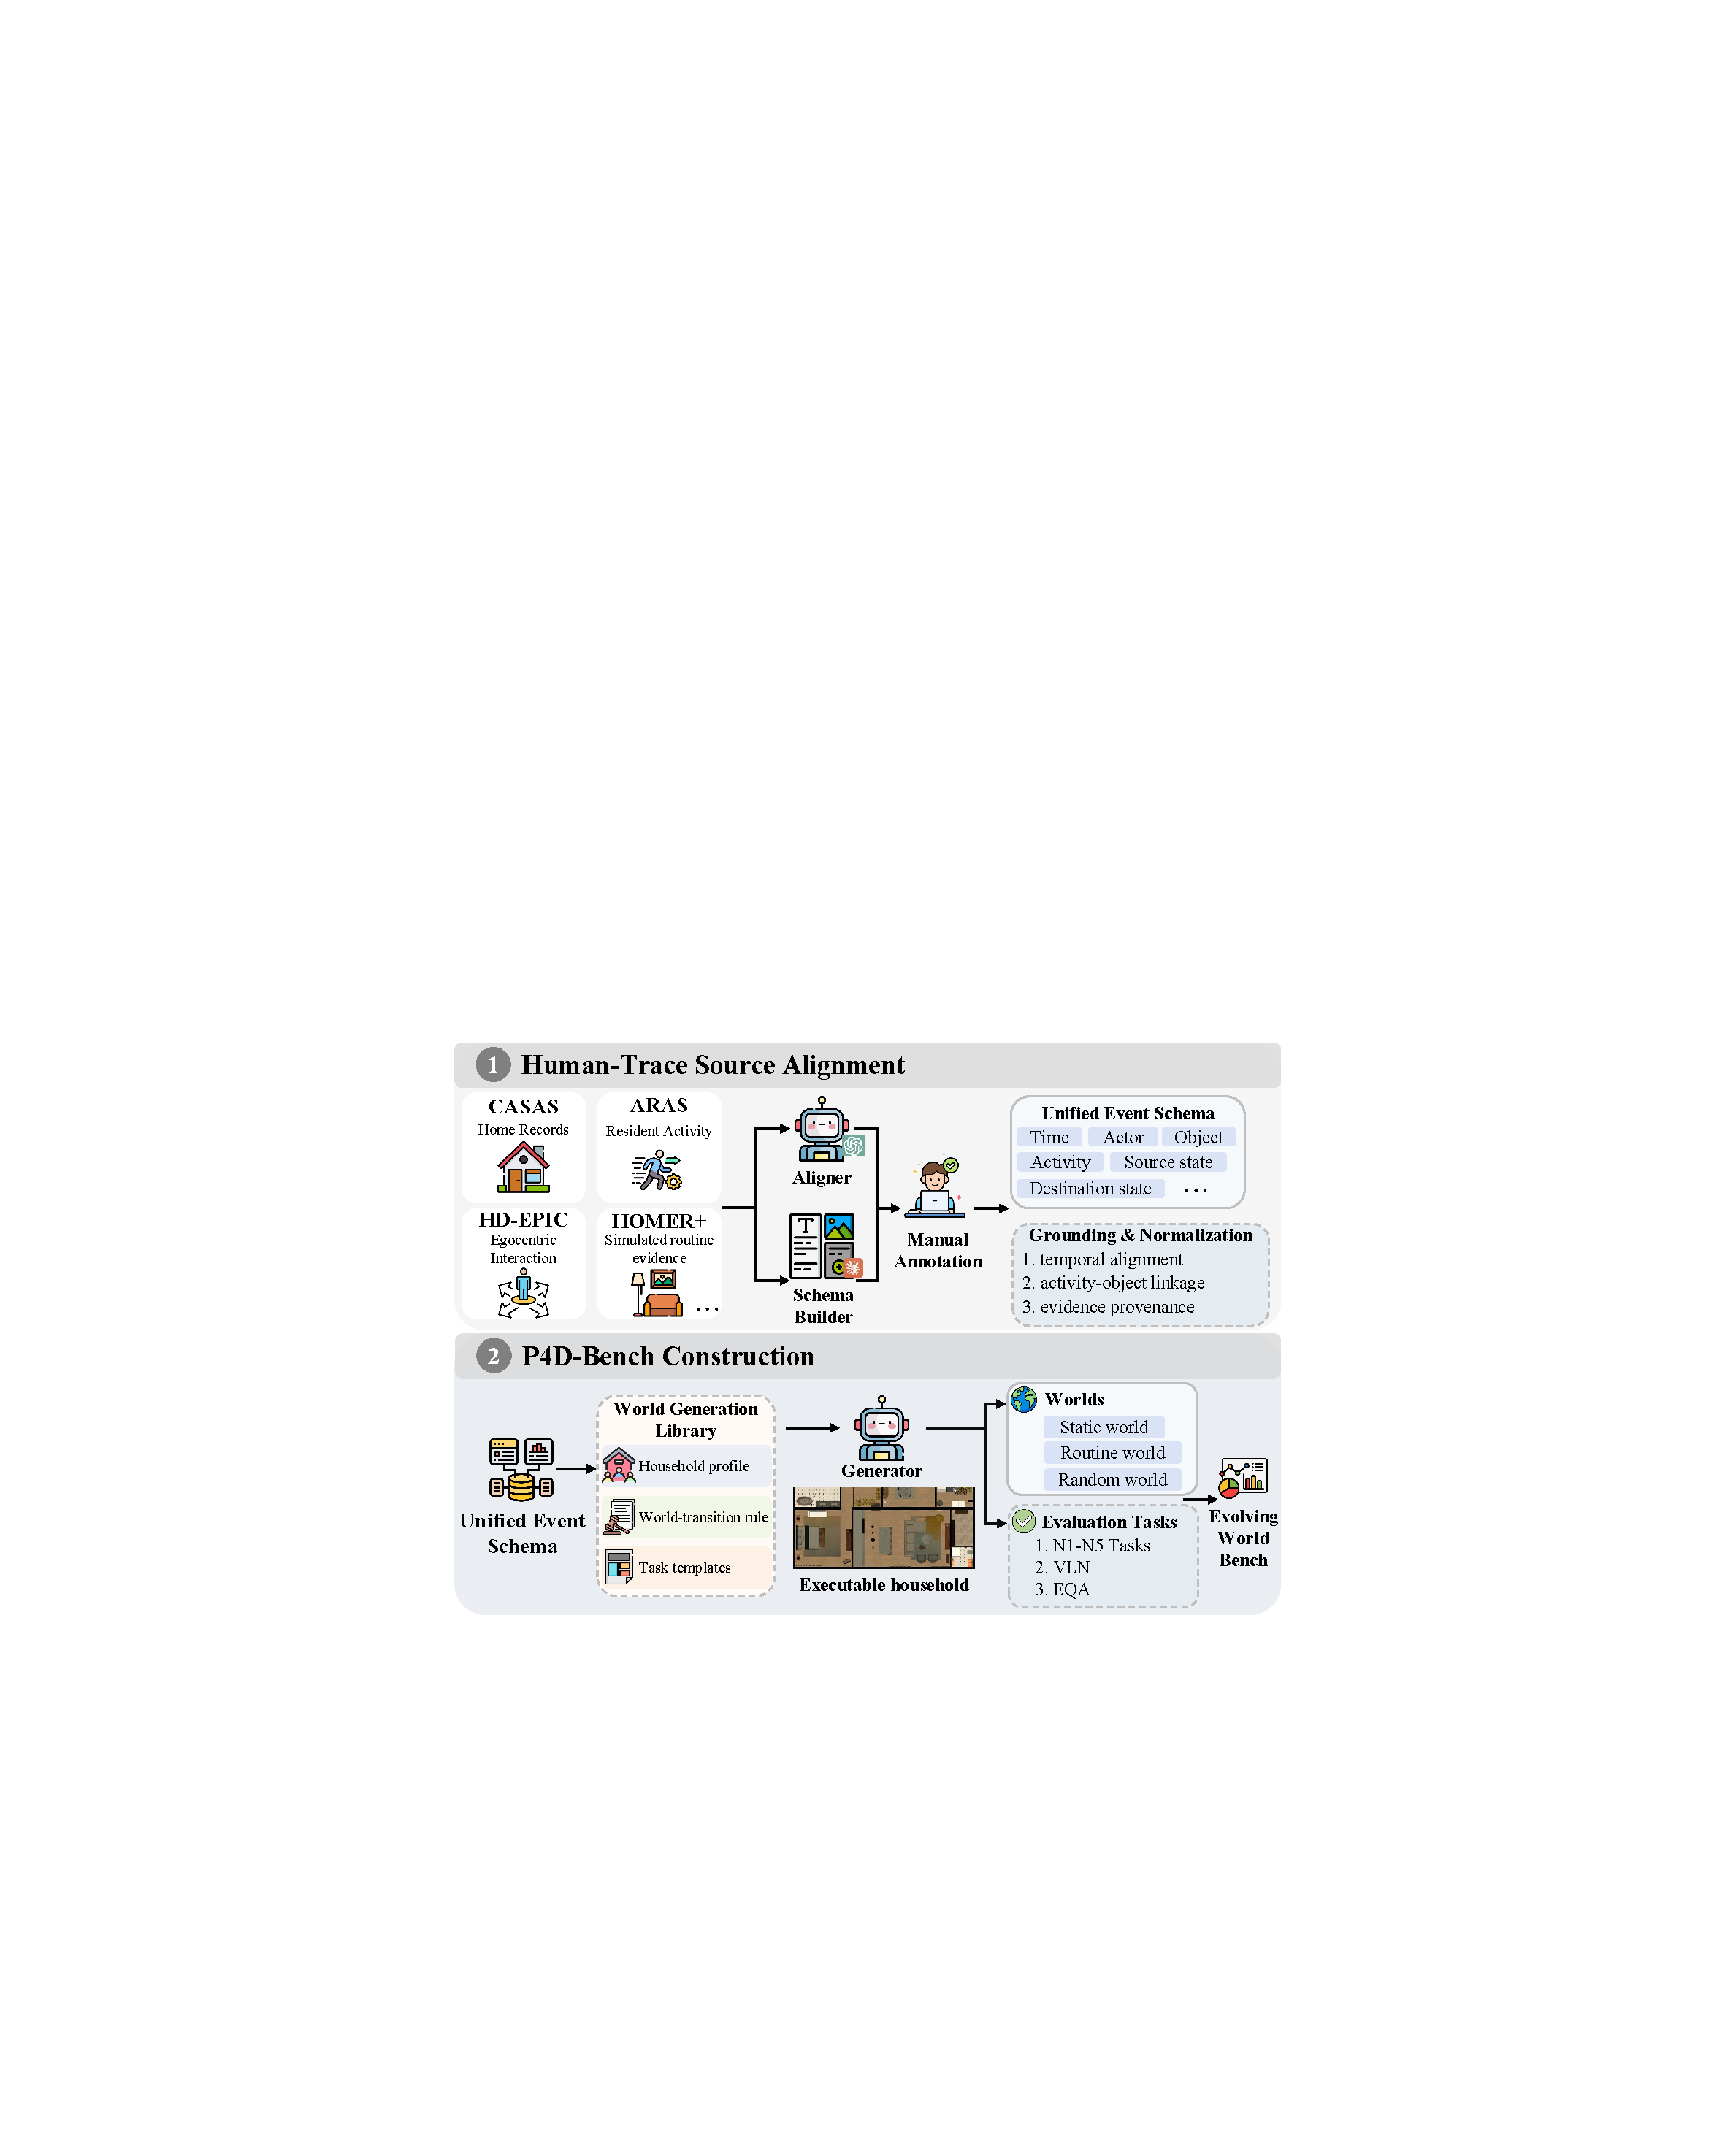
\includegraphics[width=0.80\linewidth]{figures/dataset-generate.pdf}
    \caption{Human-trace-grounded construction of \pfdbench{}.}
    \label{fig:p4dbench-generation}
\end{figure}

Across 54 HSSD scenes \citep{khanna2024hssd}, household schedules, preferences,
ownership, and placement habits are frozen while activities, resident
trajectories, and object transitions are generated chronologically
(\cref{fig:p4dbench-generation}). These persistent factors make history
informative; stochastic events and exceptions prevent deterministic scripts.
Audited histories yield 42.6 region transitions per resident-day, 6.56 relocations
per personal object-day, 52.6\% within-region relocations, and zero terminal
collisions.

\paragraph{Paired worlds.}
Targets span stable/rare, routine, personal, and irregular mobility regimes;
the labels are hidden from agents (\cref{tab:mobility-regimes}). For compatible
histories and queries, paired \emph{static}, \emph{routine}, and \emph{random}
worlds share public setup variables. Static preserves the last supported state;
routine follows the household's frozen transition process; random preserves
legal candidates and marginal movement statistics while breaking learnable
temporal dependency. Routine-specific gains therefore test historical regularity
rather than category frequency or spatial convenience.

\paragraph{Physical realization and causal observation.}
Transitions are replayed chronologically in Habitat. Each placement must be
semantically valid, collision-free, and observable from a reachable viewpoint;
recorded geometry includes geodesic cost and visibility. A robot patrol uses only
the map, time, travel cost, and its own history to collect local RGB-D snapshots
and visibility-qualified evidence. Public inputs end at $t_q$ and include
observed history, the last supported state, elapsed and calendar time, legal
candidates, and spatial context. Current states, hidden transitions, activities,
mobility labels, and oracle viewpoints remain evaluator-private.

\paragraph{Evaluation protocols.}
Prediction and navigation derive from the same target--time queries
(\cref{tab:tasks}). Prediction evaluates the current-state belief without
control. N1 permits one predicted destination (First-Go SR); N2 permits
belief-guided search (Search SR and cost); N3 updates the belief after inspection
(Recovery SR); and N4 advances the world during execution (Online Recovery SR).
N5 applies these protocols to held-out scenes and households. The main navigation
protocol freezes the target after the query. Methods receive identical public
observations, candidates, geometry, starts, controllers, and budgets; only
memory, belief, and resulting decisions differ.

\paragraph{Splits and audits.}
Complete temporal sequences are split together; held-out homes test cross-scene
generalization, and paired variants and near-duplicate transition groups remain
in the same split. Audits check future timestamps, hidden fields, answer-correlated
identifiers, duplicate groups, paired-world consistency, physical validity,
reachable goals, and patrol independence from hidden state. Results are
stratified by mobility, transition class, staleness, spatial difficulty, and split.
Construction details, task definitions, and metric implementations are provided
in \cref{app:benchmark-protocol,app:benchmark-extended-design}.
\FloatBarrier
